%%% Поля и разметка страницы %%%
\documentclass[a4paper,12pt]{article}
\usepackage{lscape}		% Для включения альбомных страниц
\pagestyle{empty}		% Не нумеровать
\usepackage[left=2cm,right=2cm,
top=3cm,bottom=1.5cm,bindingoffset=0cm]{geometry} % поля


%%% Кодировки и шрифты %%%
\usepackage{cmap}						% Улучшенный поиск русских слов в полученном pdf-файле
\usepackage[T2A]{fontenc}				% Поддержка русских букв
\usepackage[utf8]{inputenc}				% Кодировка utf8
\usepackage[english, russian]{babel}	% Языки: русский, английский



%%% Математические пакеты %%%
\usepackage{amsthm,amsfonts,amsmath,amssymb,amscd} % Математические дополнения от AMS

%%% Оформление абзацев %%%
\usepackage{indentfirst} % Красная строка

\usepackage{enumitem}
\usepackage{verbatim}
\usepackage{listings}

%%% Цвета %%%
\usepackage[usenames]{color}
\usepackage{color}
\usepackage{colortbl}

%%% Таблицы %%%
\usepackage{longtable}					% Длинные таблицы
\usepackage{multirow,makecell,array}	% Улучшенное форматирование таблиц
\usepackage{multicol}

%%% Общее форматирование
\usepackage[singlelinecheck=off,center]{caption}	% Многострочные подписи
\usepackage{soul}									% Поддержка переносоустойчивых подчёркиваний и зачёркиваний
\usepackage{icomma}

%%% Библиография %%%
\usepackage{cite} % Красивые ссылки на литературу

%%% Гиперссылки %%%
\usepackage[plainpages=false,pdfpagelabels=false]{hyperref}
\definecolor{linkcolor}{rgb}{0.9,0,0}
\definecolor{citecolor}{rgb}{0,0.6,0}
\definecolor{urlcolor}{rgb}{0,0,1}
\hypersetup{
    colorlinks, linkcolor={linkcolor},
    citecolor={citecolor}, urlcolor={urlcolor}
}

%%% Изображения %%%
\usepackage{graphicx}		% Подключаем пакет работы с графикой
\graphicspath{{images/}}	% Пути к изображениям

%%% Выравнивание и переносы %%%
\sloppy					% Избавляемся от переполнений
\clubpenalty=10000		% Запрещаем разрыв страницы после первой строки абзаца
\widowpenalty=10000		% Запрещаем разрыв страницы после последней строки абзаца

%%%Оформление блоков кода %%%
\definecolor{dkgreen}{rgb}{0,0.6,0}
\definecolor{gray}{rgb}{0.5,0.5,0.5}
\definecolor{mauve}{rgb}{0.58,0,0.82}
\lstset{frame=tb,
  language=Java,
  aboveskip=3mm,
  belowskip=3mm,
  showstringspaces=false,
  columns=flexible,
  basicstyle={\small\ttfamily},
  numbers=none,
  numberstyle=\tiny\color{gray},
  keywordstyle=\color{blue},
  commentstyle=\color{dkgreen},
  stringstyle=\color{mauve},
  breaklines=true,
  breakatwhitespace=true,
  tabsize=3
}


%%% Библиография %%%
\makeatletter
\bibliographystyle{utf8gost705u}	% Оформляем библиографию в соответствии с ГОСТ 7.0.5
\renewcommand{\@biblabel}[1]{#1.}	% Заменяем библиографию с квадратных скобок на точку:
\makeatother

%%% Колонтитулы %%%
\let\Sectionmark\sectionmark
\def\sectionmark#1{\def\Sectionname{#1}\Sectionmark{#1}}
\makeatletter
\newcommand*{\currentname}{\@currentlabelname}
\renewcommand{\@oddhead}{\it \vbox{\hbox to \textwidth%
		{\hfil Информатика и ИКТ, 11 класс\hfil\strut}\hbox to \textwidth%
		{\today \hfil Физтех-лицей\strut}\hrule}}
\makeatother




%%%%%%%%%%%%%%%%%%%%%%%%%%%%%%%%%%%%%%%%%%%%%%%%%%%%%%%%%%%%%%%%%%%%%%%%%%%%%%%%%%%
\begin{document}
\begin{center}
\Large{\textbf{Лабораторная работа по физическому моделированию №1, 16 января}}
\end{center}
На последнем практическом занятии мы с вами моделировали падение камня с некоторой высоты в поле тяжести Земли. Ответ на такую простую задачку вы могли получить и без компьютера с помощью простого аналитического вычисления. Сегодня мы рассмотрим чуть более сложную задачу: мы изучим падение с трением. Итак, в этой нехитрой работе вам предстоит промоделировать высадку десанта на вражескую территорию. :-) Высадка происходит в два этапа: десантник выпрыгивает из самолета и некоторое время падает в поле тяжести с небольшим сопротивлением воздуха, затем он раскрывает парашют, сопротивление воздуха значительно усиливается, за счет чего пасадка происходит с относительно небольшой скоростью.

\section{Без парашюта и воздуха }
Для начала проделаем то, что мы уже умеем. Пусть нет никакого сопротивления воздуха и парашюта. Нам нужно построить графики координата-время и скорость-время для свободного падения в поле тяжести $\vec{g} = 9.81 \frac{m}{s^2}$. Мы будем делать это итеративно: разобьем время на маленькие промежутки $\Delta t$ и будем вычислять скорость $\vec{v}$ и высоту $h$ в каждый момент $t + \Delta t$.
\begin{itemize}
\item Создайте программу с  названием $without\_friction.py$.
\item Проимпортируем необходимые библиотеки
\begin{lstlisting}[language=python]
import matplotlib.pyplot as plt
import numpy as np
\end{lstlisting}

\item Теперь создадим функцию, которая будет возвращать массивы времен, скоростей и координат. Что она будет принимать в качестве аргументов? Высоту, с которой начинается падение, и интервал $\Delta t$. Итак, функция выглядит следующим образом:
\begin{lstlisting}[language=python]
def Fall(height, delta_t):
  list_of_velocities =[]
  list_of_times = []
  list_of_heights = []
  # ...  
  # something happens here
  # ...
  return list_of_velocities, list_of_times, list_of_heights
\end{lstlisting}
Внутри функции вам следует вычислять координаты и скорости до тех пор, пока высота больше нуля.

\item Теперь, после того как функция написана, осталось только нарисовать графики. Например, для высоты от времени:
\begin{lstlisting}[language=python]
v, t, h = Fall(2000, 0.001)
plt.title('Fall')
plt.plot(t, h)
plt.xlabel("Time")
plt.ylabel("Height")
\end{lstlisting}
\end{itemize}
Первое упражнение закончено. Надеюсь, это было не сложно.

\section{Высадка десанта}
Ну а теперь приступим к задаче! Мы будем высаживать десантника с низколетящего бомбардировщика, летящего на высоте $h = 2000 $м. Масса десантника со снаряжением $m = 90 kg$, а высота, на которой он раскрывает парашют, --- 1000 метров. Сила действующая на десантника складывается из силы притяжения и силы сопротивления воздуха. Силу сопротивления будем определять эмпирической формулой: $$\vec{F} = -0.65 S \vec{v} |v|,$$ где $v$ --- скорость падения и $S$ --- площадь поперечного сечения. (На самом деле, численный коэффициент $0.65$ очень трудно получить из теоретических соображений, поэтому его предпочитают измерять экспериментально для различных сред. Более того, к вышеприведенной формуле нужно относиться с осторожностью, ее критерии применимости --- отдельный, не очень простой, вопрос.)
\begin{itemize}
\item Создайте отдельную программу $skydiving.py$, подключите необходимые библиотеки.
\item Создайте функцию для вычисления координат и скоростей, передавая ей в качестве параметров массу парашютиста (заметьте, что масса играет роль только тогда, когда мы "включаем" трение), начальную высоту, высоту раскрытия парашюта и интервал $\Delta t$.
\begin{lstlisting}[language=python]
def Skydive(mass, position, position_open,
                delta_t):
  list_of_velocities =[]
  list_of_times = []
  list_of_heights = []
  # ...  
  # something happens here
  # ...
  return list_of_velocities, list_of_times, list_of_heights
\end{lstlisting}
\item Что же происходит внутри функции? Опять, нужно организовать цикл, пока высота больше нуля. Внутри цикла нужно высчитывать ускорение парашютиста. Оно зависит от параметра $S$. До раскрытия парашюта $S = 0.4$ квадратных метров, после --- $S = 28$ квадратных метров. В итоге, цикл выглядит примерно так:
\begin{lstlisting}[language=python]
while height > 0:
  if (height > 1000):
    S = 0.4
    air_friction = -0.65 * S *  velocity * abs(velocity)
    ...
  else:
    S = 28
    air_friction = -0.65 * S *  velocity * abs(velocity)
    ...  
\end{lstlisting}
\item Теперь осталось только выполнить функцию при для аргументов $m = 90$, $position = 2000$, $position\_open = 1000$, $delta\_t = 0.001$ и построить график. 
\item Постройте на одном графике падение без трения и приземление с парашютом. Результат должен получится как на рисунке ниже (если ваш преподаватель нигде не налажал :-).
\end{itemize}
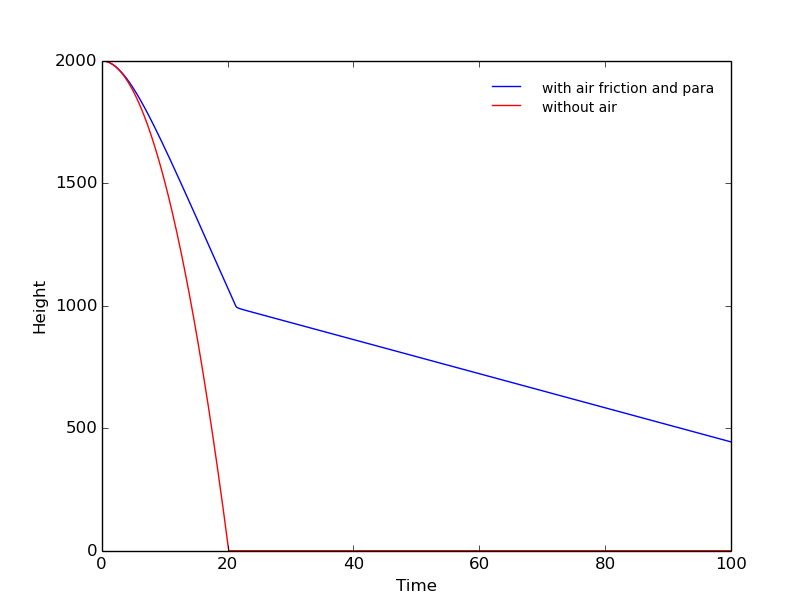
\includegraphics[scale=0.7]{skydiving}
\section{Немного рефлексии }
Остается два вопроса важных вопроса.
\begin{itemize}
\item Можете ли вы получить последний результат аналитически? Вычислите явную формулу для времени приземления парашютиста. Обязательно проделайте это полезное упражнение!
\item Очевидно, что высадку десанта на вражескую территорию нужно осуществить за как можно более короткое время. Вычислите моделированием на компьютере и аналитически, на какой высоте нужно раскрыть парашют, чтобы приземлиться как можно быстрее, считая, что критическая скорость, на которой десантник может приземлиться без повреждений, равна 10 м/c.


Как всегда, присылайте работы на почты $dontwritehim@gmail.com$ и $i\_khisambeev@mail.ru$.
\end{itemize}
\end{document}